\subsection{Multidimensionale Arrays}
Intern ist ein multidimensionales Array im Prinzip das gleiche wie ein lineares Array.

Da der Speicher eines Rechners linear ist, ist es ein eindimensionales Array.
Zur Vereinfachung kann dieses multidimensionales Array leicht als eindimensional dargestellt werden.

Beispielsweise werden die Elemente eines 3x4 Arrays folgendermaßen in einem eindimensionalen Array aus 12 Zellen
gespeichert:

% TODO FIXME not clear. First, horizontal would be better. Second, why two columns?
% I'd first show 3x4 with numbered elements (e.g. 32-bit ints) in colored lines,
% then linear with the same numbered elements (and colored blocks)
% then linear with addresses (offsets) - assuming let say 32-bit ints.
\begin{table}[H]
\centering
\begin{tabular}{ | l | l | }
\hline
Offset im Speicher & Arrayelement \\
\hline
0 & [0][0] \\
\hline
1 & [0][1] \\
\hline
2 & [0][2] \\
\hline
3 & [0][3] \\
\hline
4 & [1][0] \\
\hline
5 & [1][1] \\
\hline
6 & [1][2] \\
\hline
7 & [1][3] \\
\hline
8 & [2][0] \\
\hline
9 & [2][1] \\
\hline
10 & [2][2] \\
\hline
11 & [2][3] \\
\hline
\end{tabular}
\caption{Zweidimensionales Array in eindimensionaler Speicherdarstellung}
\end{table}

Auf diese Weise wird jede Zellen des 3*4 Arrays im Speicher abgelegt:

% TODO coordinates. TikZ?
\begin{table}[H]
\centering
\begin{tabular}{ | l | l | l | l | }
\hline                        
0 & 1 & 2 & 3 \\
\hline  
4 & 5 & 6 & 7 \\
\hline  
8 & 9 & 10 & 11 \\
\hline  
\end{tabular}
\caption{Speicheradressen jeder Zelle des zweidimensionalen Arrays}
\end{table}

\myindex{row-major order}
Um also die Adresse des benötigten Elements zu berechnen, multiplizieren wir zunächst den ersten Index mit 4 (der
Arraybreite) und addieren dann den zweiten Index.
Dies nennt man \emph{Zeilenordnung} (engl. row-major order) und diese Methode zur Darstellung von Arrays und Matrizen
wird mindestens von \CCpp und Python verwendet.
Der Ausdruck row-major order bedeutet: \q{schreibe zuerst die Elemente der ersten Zeilen, dann die zweite Zeile\dots
und schließlich die Elemente der letzten Zeile}.

\myindex{column-major order}
\myindex{Fortran}
Eine andere Methode zur Darstellung heißt \emph{Spaltenordnung} (engl. column-major order) (die Indizes des Arrays werden
in umgekehrter Reihenfolge verwendet) und wird zumindest in Fortran, MATLAB und R verwendet.
Der Ausdruck column-major oder bedeutet: \q{schreibe zuerst die Elemente der ersten Spalte, dann die zweite Spalte\dots
und schließlich die Elemente der letzten Spalte}.

Welche Method ist besser?

Generel ist hinsichtlich Performance und Cachespeicher die beste Methode der Datenorganisation diejenige, in der auf die
Elemente sequentiell zugegriffen wird.

Wenn eine Funktion auf Daten zeilenweise zugreift, ist Zeilenordnung besser und umgekehrt.

% subsubsections
\subsubsection{Beispiel für zweidimensionales Array}
Wir werden mit einem Array vom Typ \Tchar arbeiten, was bedeutet, dass jedes Element nur ein Byte Speicherplatz
benötigt.


\myparagraph{Beispiel: Zeile füllen}
\myindex{\olly}
Füllen wir die zweite Zeilen mit den Werten 0..3:

\lstinputlisting[caption=Row filling example,style=customc]{patterns/13_arrays/5_multidimensional/two1_DE.c}
Alle drei Zeilen sind rot markiert.
Wir erkennen, dass die zweite Zeilen nun die Werte 0,1,2 und 3 enthält:

\begin{figure}[H]
\centering
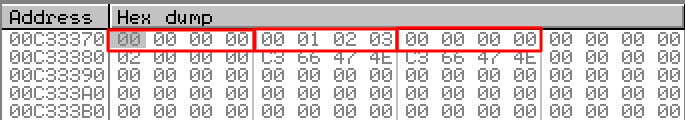
\includegraphics[width=0.6\textwidth]{patterns/13_arrays/5_multidimensional/olly_2D_1.png}
\caption{\olly: Array ist befüllt}
\end{figure}

\myparagraph{Beipsiel: Spalte füllen}
\myindex{\olly}
Füllen wir die dritte Spalte mit den Werten 0..2:

\lstinputlisting[caption=Column filling example,style=customc]{patterns/13_arrays/5_multidimensional/two2_DE.c}

Die drei Spalten sind hier ebenfalls rot markiert.

Wir erkennen, dass sich in jeder Zeile an der dritten Stelle die Werte 0,1 und 2 befinden. 

\begin{figure}[H]
\centering
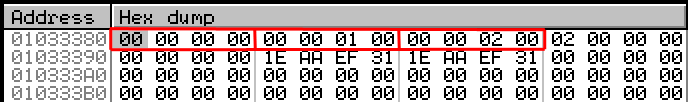
\includegraphics[width=0.6\textwidth]{patterns/13_arrays/5_multidimensional/olly_2D_2.png}
\caption{\olly: Array ist befüllt}
\end{figure}


\subsubsection{Eindimensionaler Zugriff auf zweidimensionales Array}
Wir können uns leicht davon überzeugen, dass es auf mindestens zwei Arten möglich ist, auf ein zweidimensionales Array
eindimensional zuzugreifen:

\lstinputlisting[style=customc]{patterns/13_arrays/5_multidimensional/2D_as_1D_DE.c}

% TBT
Kompilieren und ausführen: es zeigt korrekte Werte an
Was MSVC 2013 getan hat ist faszinierend: alle drei Routinen sind identisch!

\lstinputlisting[caption=\Optimizing MSVC 2013 x64,style=customasmx86]{patterns/13_arrays/5_multidimensional/2D_as_1D_MSVC_2013_Ox_x64_DE.asm}

GCC erzeugt ebenfalls äquivalente Routinen, aber ein wenig anders:

\lstinputlisting[caption=\Optimizing GCC 4.9 x64,style=customasmx86]{patterns/13_arrays/5_multidimensional/2D_as_1D_GCC49_x64_O3_DE.s}


\subsubsection{Beispiel: dreidimensionales Array}

Mit multidimensionalen Arrays ist es das gleiche.

Wir werden nun mit einem Array vom Typ \Tint arbeiten: jedes Element benötigt 4 Byte Speicherplatz.

Sehen wir es uns an:

\lstinputlisting[caption=simple example,style=customc]{patterns/13_arrays/5_multidimensional/multi.c}

\myparagraph{x86}

Wir erhalten das Folgende (MSVC 2010):

\lstinputlisting[caption=MSVC 2010,style=customasmx86]{patterns/13_arrays/5_multidimensional/multi_msvc_DE.asm}
Nichts Außergewöhnliches. Zur Berechnung des Index' werden in der Formel $address=600 \cdot 4 \cdot x + 30 \cdot 4 \cdot
y + 4z$ drei Eingabewerte verwendet, um das multidimensionale Array zu repräsentieren.
Vergessen wir nicht, dass der \Tint Typ 32 Bit (4 Byte) breit ist, sodass alle Koeffizienten mit 4 multipliziert werden
müssen.

\lstinputlisting[caption=GCC 4.4.1,style=customasmx86]{patterns/13_arrays/5_multidimensional/multi_gcc_DE.asm}
Der GCC Compiler arbeitet anders.

Für eine der Operationen in der Berechnung ($30y$) produziet GCC Code ohne Multiplikationsbefehle.
Das funktioniert wie folgt:
$(y+y) \ll 4 - (y+y) = (2y) \ll 4 - 2y = 2 \cdot 16 \cdot y - 2y = 32y - 2y = 30y$.

So werden für die $30y$ Berechnung nur ein Addierbefehl, eine bitweiser Verschiebebefehl und ein Subtraktionsbefehl
verwendet. So geht es schneller.

\myparagraph{ARM + \NonOptimizingXcodeIV (\ThumbMode)}

\lstinputlisting[caption=\NonOptimizingXcodeIV (\ThumbMode),style=customasmARM]{patterns/13_arrays/5_multidimensional/multi_Xcode_thumb_O0_DE.asm}

\NonOptimizing LLVM speichert alle Variablen auf dem lokalen Stack, was redundant ist.

Die Adresse des Arrayelements wird über die eben gezeigte Formel berechnet.

\myparagraph{ARM + \OptimizingXcodeIV (\ThumbMode)}

\lstinputlisting[caption=\OptimizingXcodeIV (\ThumbMode),style=customasmARM]{patterns/13_arrays/5_multidimensional/multi_Xcode_thumb_O3_DE.asm}
Die Tricks für das Ersetzen der Multiplikation durch Verschieben, Addieren und Subtrahieren, die wir bereits
kennengelernt haben, kommen hier auch vor.

\myindex{ARM!\Instructions!RSB}
\myindex{ARM!\Instructions!SUB}
Hier finden wir auch einen für uns neuen Befehl: \RSB (\emph{Reverse Subtract}).

Er arbeitet genau wie \SUB, aber vertauscht die Operanden vor der Ausführung. Warum?

\myindex{ARM!Optional operators!LSL}
\SUB und \RSB  sind Befehle, bei denen auf den zweiten Operanden eine bitweise Verschiebung angewendet werden kann:
(\INS{LSL\#4}).
Dieser Koeffizient kann aber nur auf den zweiten Operanden angewendet werden.

Das ist günstig für kommutative Operationen wie Addition und Multiplikation (die Operanden können vertauscht werden,
ohne das Ergebnis zu verändern).

Subtraktion dagegen ist nicht kommutativ, weshalb für diese Fälle \RSB existiert.

\myparagraph{MIPS}

\myindex{MIPS!Global Pointer}
Das Beispiel ist sehr klein, sodass der GCC Compiler entschieden hat das Array $a$ im 64KiB Platz abzulegen, um es durch
den globalen Pointer zugreifbar zu machen.

\lstinputlisting[caption=\Optimizing GCC 4.4.5 (IDA),style=customasmMIPS]{patterns/13_arrays/5_multidimensional/multi_MIPS_O3_IDA_DE.lst}


% \input{patterns/13_arrays/5_multidimensional/dimensions_DE}

\subsubsection{Weitere Beispiele}
Der Bildschirm wird als 2D-Array dargestellt, aber der Videopuffer ist ein lineares 1D-Array.
Wir betrachten hier näher: \myref{Mandelbrot_demo}.

Ein anderes Beispiel in diesem Buch ist das Spiel Minesweeper: das Feld ist auch ein zweidimensionales Array:
\myref{minesweeper_winxp}.

